\documentclass[journal,12pt,twocolumn]{IEEEtran}
%
\usepackage{setspace}
\usepackage{gensymb}
\usepackage{siunitx}
\usepackage{tkz-euclide} 
\usepackage{textcomp}
\usepackage{standalone}
\usetikzlibrary{calc}

%\doublespacing
\singlespacing

%\usepackage{graphicx}
%\usepackage{amssymb}
%\usepackage{relsize}
\usepackage[cmex10]{amsmath}
%\usepackage{amsthm}
%\interdisplaylinepenalty=2500
%\savesymbol{iint}
%\usepackage{txfonts}
%\restoresymbol{TXF}{iint}
%\usepackage{wasysym}
\usepackage{amsthm}
%\usepackage{iithtlc}
\usepackage{mathrsfs}
\usepackage{txfonts}
\usepackage{stfloats}
\usepackage{bm}
\usepackage{cite}
\usepackage{cases}
\usepackage{subfig}
%\usepackage{xtab}
\usepackage{longtable}
\usepackage{multirow}
%\usepackage{algorithm}
%\usepackage{algpseudocode}
\usepackage{enumitem}
\usepackage{mathtools}
\usepackage{steinmetz}
\usepackage{tikz}
\usepackage{circuitikz}
\usepackage{verbatim}
\usepackage{tfrupee}
\usepackage[breaklinks=true]{hyperref}
%\usepackage{stmaryrd}
\usepackage{tkz-euclide} % loads  TikZ and tkz-base
%\usetkzobj{all}
\usetikzlibrary{calc,math}
\usepackage{listings}
    \usepackage{color}                                            %%
    \usepackage{array}                                            %%
    \usepackage{longtable}                                        %%
    \usepackage{calc}                                             %%
    \usepackage{multirow}                                         %%
    \usepackage{hhline}                                           %%
    \usepackage{ifthen}                                           %%
  %optionally (for landscape tables embedded in another document): %%
    \usepackage{lscape}     
\usepackage{multicol}
\usepackage{chngcntr}
\usepackage{amsmath}
\usepackage{cleveref}
%\usepackage{enumerate}

%\usepackage{wasysym}
%\newcounter{MYtempeqncnt}
\DeclareMathOperator*{\Res}{Res}
%\renewcommand{\baselinestretch}{2}
\renewcommand\thesection{\arabic{section}}
\renewcommand\thesubsection{\thesection.\arabic{subsection}}
\renewcommand\thesubsubsection{\thesubsection.\arabic{subsubsection}}

\renewcommand\thesectiondis{\arabic{section}}
\renewcommand\thesubsectiondis{\thesectiondis.\arabic{subsection}}
\renewcommand\thesubsubsectiondis{\thesubsectiondis.\arabic{subsubsection}}

% correct bad hyphenation here
\hyphenation{op-tical net-works semi-conduc-tor}
\def\inputGnumericTable{}                                 %%

\lstset{
%language=C,
frame=single, 
breaklines=true,
columns=fullflexible
}
%\lstset{
%language=tex,
%frame=single, 
%breaklines=true
%}
\usepackage{graphicx}
\usepackage{pgfplots}

\begin{document}
%


\newtheorem{theorem}{Theorem}[section]
\newtheorem{problem}{Problem}
\newtheorem{proposition}{Proposition}[section]
\newtheorem{lemma}{Lemma}[section]
\newtheorem{corollary}[theorem]{Corollary}
\newtheorem{example}{Example}[section]
\newtheorem{definition}[problem]{Definition}
%\newtheorem{thm}{Theorem}[section] 
%\newtheorem{defn}[thm]{Definition}
%\newtheorem{algorithm}{Algorithm}[section]
%\newtheorem{cor}{Corollary}
\newcommand{\BEQA}{\begin{eqnarray}}
\newcommand{\EEQA}{\end{eqnarray}}
\newcommand{\define}{\stackrel{\triangle}{=}}
\bibliographystyle{IEEEtran}
%\bibliographystyle{ieeetr}
\providecommand{\mbf}{\mathbf}
\providecommand{\pr}[1]{\ensuremath{\Pr\left(#1\right)}}
\providecommand{\qfunc}[1]{\ensuremath{Q\left(#1\right)}}
\providecommand{\sbrak}[1]{\ensuremath{{}\left[#1\right]}}
\providecommand{\lsbrak}[1]{\ensuremath{{}\left[#1\right.}}
\providecommand{\rsbrak}[1]{\ensuremath{{}\left.#1\right]}}
\providecommand{\brak}[1]{\ensuremath{\left(#1\right)}}
\providecommand{\lbrak}[1]{\ensuremath{\left(#1\right.}}
\providecommand{\rbrak}[1]{\ensuremath{\left.#1\right)}}
\providecommand{\cbrak}[1]{\ensuremath{\left\{#1\right\}}}
\providecommand{\lcbrak}[1]{\ensuremath{\left\{#1\right.}}
\providecommand{\rcbrak}[1]{\ensuremath{\left.#1\right\}}}
\theoremstyle{remark}
\newtheorem{rem}{Remark}
\newcommand{\sgn}{\mathop{\mathrm{sgn}}}
\providecommand{\abs}[1]{\left\vert#1\right\vert}
\providecommand{\res}[1]{\Res\displaylimits_{#1}} 
\providecommand{\norm}[1]{\left\lVert#1\right\rVert}
%\providecommand{\norm}[1]{\lVert#1\rVert}
\providecommand{\mtx}[1]{\mathbf{#1}}
\providecommand{\mean}[1]{E\left[ #1 \right]}
\providecommand{\fourier}{\overset{\mathcal{F}}{ \rightleftharpoons}}
%\providecommand{\hilbert}{\overset{\mathcal{H}}{ \rightleftharpoons}}
\providecommand{\system}{\overset{\mathcal{H}}{ \longleftrightarrow}}
	%\newcommand{\solution}[2]{\textbf{Solution:}{#1}}
\newcommand{\solution}{\noindent \textbf{Solution: }}
\newcommand{\cosec}{\,\text{cosec}\,}
\providecommand{\dec}[2]{\ensuremath{\overset{#1}{\underset{#2}{\gtrless}}}}
\newcommand{\myvec}[1]{\ensuremath{\begin{pmatrix}#1\end{pmatrix}}}
\newcommand{\mydet}[1]{\ensuremath{\begin{vmatrix}#1\end{vmatrix}}}
%\numberwithin{equation}{section}
\numberwithin{equation}{subsection}
%\numberwithin{problem}{section}
%\numberwithin{definition}{section}
\makeatletter
\@addtoreset{figure}{problem}
\makeatother
\let\StandardTheFigure\thefigure
\let\vec\mathbf
%\renewcommand{\thefigure}{\theproblem.\arabic{figure}}
\renewcommand{\thefigure}{\theproblem}
%\setlist[enumerate,1]{before=\renewcommand\theequation{\theenumi.\arabic{equation}}
%\counterwithin{equation}{enumi}
%\renewcommand{\theequation}{\arabic{subsection}.\arabic{equation}}
\def\putbox#1#2#3{\makebox[0in][l]{\makebox[#1][l]{}\raisebox{\baselineskip}[0in][0in]{\raisebox{#2}[0in][0in]{#3}}}}
     \def\rightbox#1{\makebox[0in][r]{#1}}
     \def\centbox#1{\makebox[0in]{#1}}
     \def\topbox#1{\raisebox{-\baselineskip}[0in][0in]{#1}}
     \def\midbox#1{\raisebox{-0.5\baselineskip}[0in][0in]{#1}}
\vspace{3cm}
\title{Matrix Theory (EE5609) Assignment 7}
\author{Arkadipta De\\MTech Artificial Intelligence\\AI20MTECH14002}

\maketitle
\newpage
%\tableofcontents
\bigskip
\renewcommand{\thefigure}{\theenumi}
\renewcommand{\thetable}{\theenumi}

\begin{abstract}
This finds whether a given second degree equation represents a pair of straight lines or not.
\end{abstract}

All the codes for the figure in this document can be found at
\begin{lstlisting}
https://github.com/Arko98/EE5609/blob/master/Assignment_7
\end{lstlisting}

\section{Problem}
Find the value of $k$ so that the following equation may represent a pair of straight lines - 
\begin{align*}
6x^2 +xy+ky^2-11x+43y-35 = 0
\end{align*}
\section{Theory}
The general equation of second degree is given
by,
\begin{align}
ax^2+2bxy+cy^2+2dx+2ey+f = 0\label{eq1}\\
\intertext{\eqref{eq1} can be written as,}\\
\vec{x^TVx} + 2\vec{u^Tx} + f = 0\label{eq2}
\intertext{where,}
\vec{V} = \vec{V^T} = \myvec{a&b\\b&c}\\
\vec{u} = \myvec{d\\e}
\intertext{\eqref{eq2} represents a pair of straight lines if,}
\mydet{\vec{V}&\vec{u}\\\vec{u^T}&f} = 0\label{eq3}
\end{align}
Otherwise, \eqref{eq2} represents a conic section.
\section{Solution}

\begin{comment}

\begin{figure}[!h]
\centering
\resizebox{\columnwidth}{!}{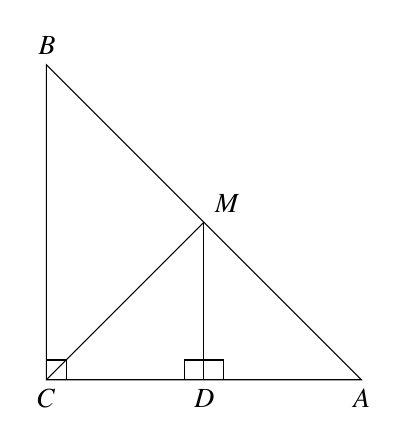
\begin{tikzpicture}
\coordinate (B) at (0,4);
\coordinate (A) at (4,0);
\coordinate (C) at (0,0);
\coordinate (D) at (2,0);
\coordinate (M) at (2,2);
\draw (A)node[below]{$A$}--(B)node[above]{$B$}--(C)node[below]{$C$}--cycle;
\draw(M)node[above right]{$M$}--(D)node[below]{$D$};
\draw(M)--(D);
\draw(M)--(C);
\tkzMarkRightAngle(B,C,A)
\tkzMarkRightAngle(A,D,M)
\tkzMarkRightAngle(C,D,M)
\end{tikzpicture}
}
\caption{Right Angled Triangle by Latex-Tikz}
\label{myfig}
\end{figure}
\end{comment}
The given second degree equation is,
\begin{align}
6x^2 +xy+ky^2-11x+43y-35 = 0 \label{eq4}
\end{align}
Comparing coefficients of \eqref{eq4} with \eqref{eq1} we get,
\begin{align}
\vec{V} &= \myvec{6&\frac{1}{2}\\\frac{1}{2}&k}\\
\vec{u} &= \myvec{-\frac{11}{2}\\\frac{43}{2}}\\
f &= -35
\end{align}

From \eqref{eq3} the given second degree equation \eqref{eq4} will represent a pair of straight line if, 
\begin{align}
\mydet{6&\frac{1}{2}&-\frac{11}{2}\\ \frac{1}{2}&k&\frac{43}{2}\\-\frac{11}{2}& \frac{43}{2}&-35}&=0\\
\intertext{Expanding the determinant,}
k+12&=0\\
\implies k&=-12\label{eq5}
\end{align}
Hence, from \eqref{eq5} we find that for $k=-12$, the given second degree equation \eqref{eq4} represents pair of straight lines. For the appropriate value of $k$, \eqref{eq4} becomes,
\begin{align}
6x^2 +xy-12y^2-11x+43y-35 = 0\label{eqmain}
\end{align}

\section{Graphical Illustration}
We obtain the linear equation of the form ($ax + by + c$) from \eqref{eqmain} by considering
\begin{align}
6x^2 + xy - 12y^2 &= 6x^2 - 8xy + 9xy - 12y^2\\
&= 2x(3x - 4y) + 3y(3x - 4y)\\
&= (3x - 4y)(2x + 3y) \label{eqmain2}
\end{align}
Again \eqref{eqmain} can be written using \eqref{eqmain2} as,
\begin{align}
(3x-4y+m)(2x+3y+n)&=0 \label{eqSubs} \\
\implies 6x^2+ xy-12y^2+(2m+3n)x\nonumber\\+(3m-4n)y+mn &= 0 \label{eqmain3}
\end{align}
Equating coefficients of \eqref{eq4} and \eqref{eqmain3},
\begin{align}
2m+3n &= -11\\
3m-4n &= 43
\intertext{The equations can be written as follows,}
\myvec{2&3\\3&-4}\myvec{m\\n}&=\myvec{-11\\43}\label{eqmain4}
\end{align}
The augmented matrix of \eqref{eqmain4} is,
\begin{align}
\myvec{2&3&-11\\3&-4&43}\underleftrightarrow{R_1=\frac{1}{2}R_1}\myvec{1&\frac{3}{2}&-\frac{11}{2}\\3&-4&43}\\
\underleftrightarrow{R_2=R_2-3R_1}\myvec{1&\frac{3}{2}&-\frac{11}{2}\\0&-\frac{17}{2}&\frac{119}{2}}\\
\underleftrightarrow{R_2=-\frac{2}{17}R_2}\myvec{1&\frac{3}{2}&-\frac{11}{2}\\0&1&-7}\\
\underleftrightarrow{R_1=R_1-\frac{3}{2}R_2}\myvec{1&0&5\\0&1&-7}\\
\end{align}
Hence we get,
\begin{align}
	m &= 5 \label{eqsol1} \\
	n &= -7 \label{eqsol2}
\end{align}
Substituting \eqref{eqsol1} and \eqref{eqsol2} in \eqref{eqSubs}, we obtain
\begin{align}
	(3x - 4y + 5)(2x + 3y - 7) = 0 \label{eqfinal}
\end{align}
Hence \eqref{eqfinal} represents equation of a pair of straight lines.\\
The figure below corresponds to the pair of straight lines represented by \eqref{eqfinal}.
\renewcommand{\thefigure}{1}
\begin{figure}[h!]
\centering
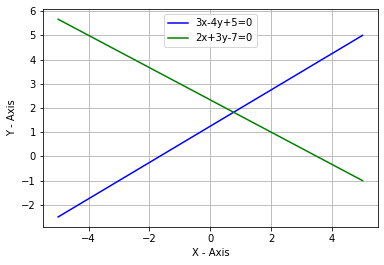
\includegraphics[width = \columnwidth]{Lines.png}
\caption{Pair of Straight Lines}
\label{fig:my_label}
\end{figure}
\end{document}
